\chapter{Requirements Analysis and Data Specification}

\section*{Introduction}
\phantomsection
\addcontentsline{toc}{section}{Introduction}

\section{Requirements Modelling}

\subsection{Use-Case Diagram}
\subsubsection{Global Use Case Diagram}

The figure below presents the global use case diagram for the content creator, showing all major functionalities accessible from the dashboard.

% ── FIGURE: Global use case diagram ──
 \begin{figure}[H]
     \centering
     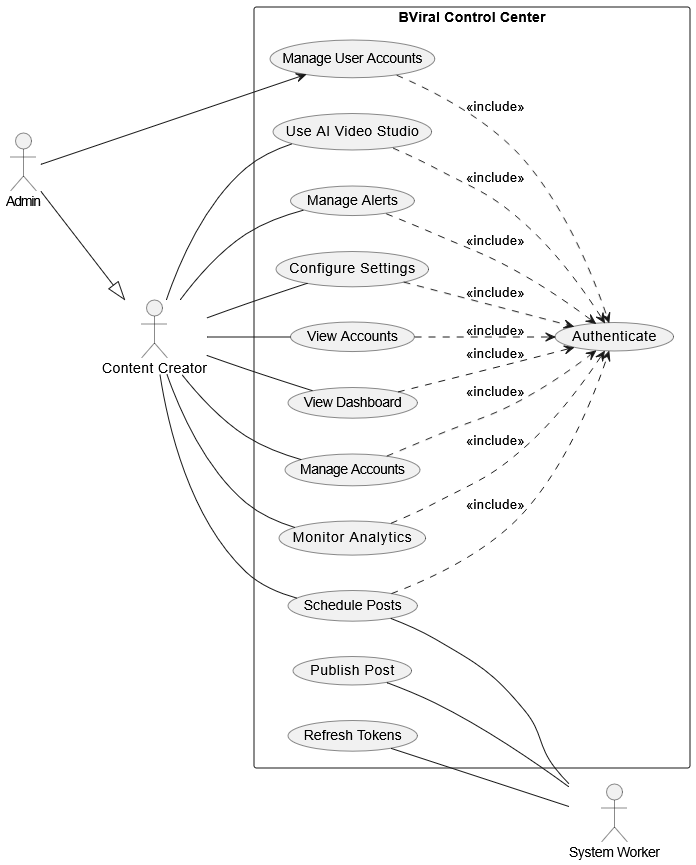
\includegraphics[width=0.65\textwidth]{diagram/diagram1.png}
     \caption{Global use case diagram for the Content Creator and admin}
     \label{fig:uc-global}
 \end{figure}

\vspace{0.5cm}

The content creator and admin interact with the following subsystems after authentication:
\begin{itemize}
    \item Dashboard overview (KPIs and statistics)
    \item Account management (connect/disconnect platforms)
    \item Post scheduling (create, view, cancel posts)
    \item Analytics monitoring
    \item AI Video Studio (enhance and edit videos)
    \item Alert management
    \item System settings
\end{itemize}

In addition, the admin has exclusive privileges for user management. Specifically, the admin is responsible for managing content creator accounts, including creating new accounts, updating user information, deleting accounts, and controlling access permissions. This ensures proper system governance, security, and centralized control over platform users.
%subsubsection*{Use Case Diagram: Account Management}

 \begin{figure}[H]
     \centering
     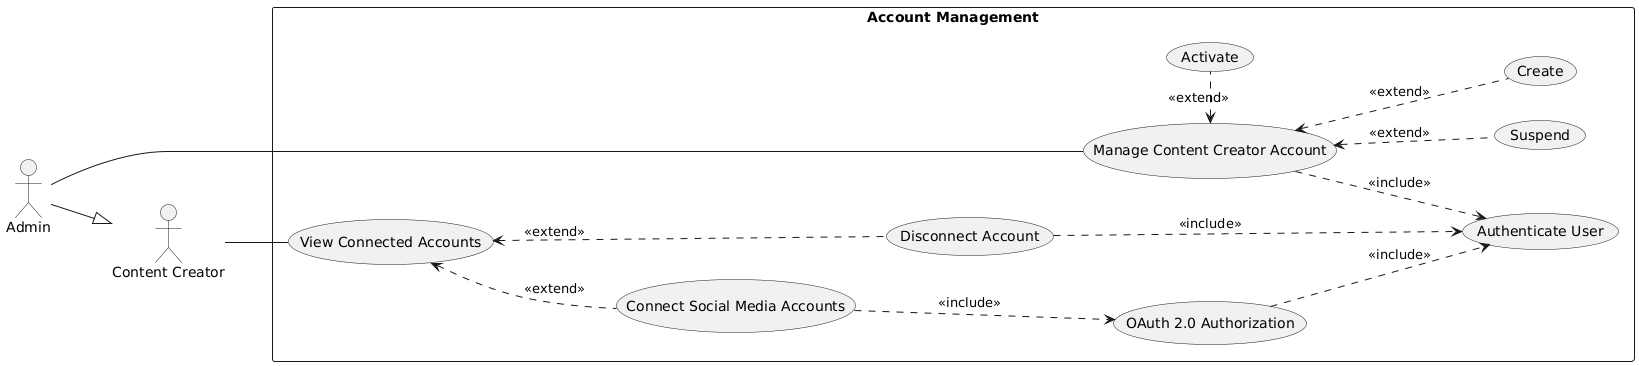
\includegraphics[width=0.95\textwidth]{diagram/diagram 2.png}
     \caption{Use case diagram of ``Account Management''}
     \label{fig:uc-accounts}
 \end{figure}

 \begin{table}[H]
\centering
\renewcommand{\arraystretch}{1.4}
\begin{tabular}{|p{4cm}|p{10cm}|}
\hline
\textbf{Title} & Account Management \\ \hline

\textbf{Actor} & Content Creator / Admin \\ \hline

\textbf{Summary} & 
This use case allows the actor to manage connected social media accounts and content creator accounts. \\ \hline

\textbf{Precondition} & 
The actor must be authenticated. \\ \hline

\textbf{Postcondition} & 
Accounts are successfully connected, modified, viewed, or deleted. \\ \hline

\textbf{Main Scenario} & 
- The actor accesses the account management module \newline
- The system displays the connected accounts \newline
- The actor can connect a new social media account \newline
- The system performs OAuth 2.0 authorization \newline
- The actor can view or disconnect an account \newline
- The admin can manage content creator accounts \newline
- The system saves the performed changes \\ \hline

\textbf{Alternative Scenario} & 
- Authentication failure \newline
- OAuth 2.0 authorization failure \newline
- Social media account already connected \newline
- Error while deleting or modifying an account \\ \hline

\end{tabular}
\caption{Use Case Description — Account Management}
\label{tab:account-management}
\end{table}

%\subsubsection*{Use Case Diagram: Post Scheduling}

 \begin{figure}[H]
     \centering
     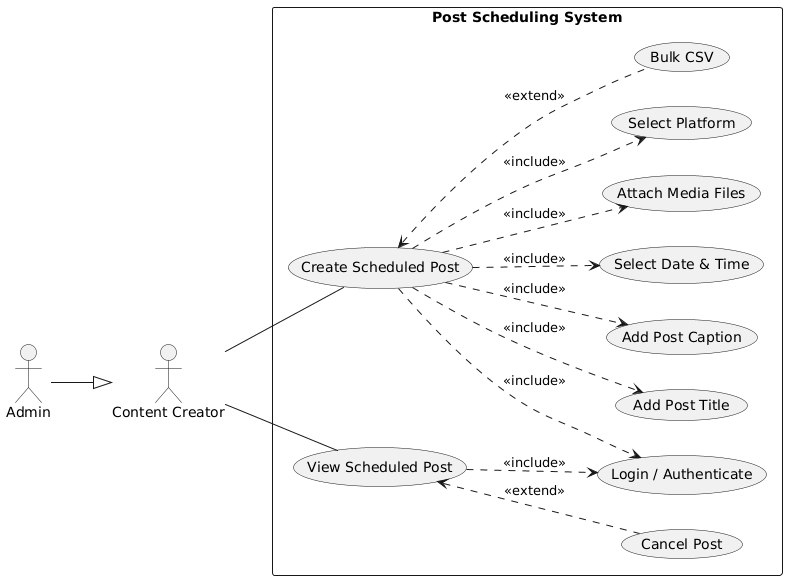
\includegraphics[width=0.75\textwidth]{diagram/diagram 3.png}
     \caption{Use case diagram of ``Post Scheduling''}
     \label{fig:uc-analytics}
 \end{figure}

%\noindent\textit{See StarUML code --- Diagram 3.}

\begin{table}[H]
\centering
\renewcommand{\arraystretch}{1.4}
\begin{tabular}{|p{4cm}|p{10cm}|}
\hline
\textbf{Title} & Post Scheduling System \\ \hline

\textbf{Actor} & Content Creator / Admin \\ \hline

\textbf{Summary} & 
This use case allows the actor to create, schedule, view, and cancel social media posts. \\ \hline

\textbf{Precondition} & 
The actor must be authenticated. \\ \hline

\textbf{Postcondition} & 
The post is successfully scheduled, viewed, or canceled. \\ \hline

\textbf{Main Scenario} & 
- The actor accesses the post scheduling module \newline
- The actor must authenticate \newline
- The actor creates a scheduled post \newline
- The actor must add post title\newline
- The actor must add post caption\newline
- The actor must select the target platform \newline
- The actor must select the publication date and time \newline
- The actor must attache media files \newline
- The actor must save the scheduled post \newline
- The actor can view scheduled posts \newline
-The System Worker actor automatically publishes posts at their scheduled time
using BullMQ queues\newline
- The actor can Bulk CSV \\ \hline

\textbf{Alternative Scenario} & 
- Authentication failure \newline
- Invalid publication date or time \newline
- Unsupported media file format \newline
- Failure while uploading media files \newline
- Error while canceling the scheduled post \newline
- Bulk CSV import contains invalid data \\ \hline

\end{tabular}
\caption{Use Case Description — Post Scheduling System}
\label{tab:post-scheduling-system}
\end{table}


%\noindent\textit{See StarUML code --- Diagram 5.}
\subsubsection*{Use Case Diagram: Use Ai studio}
 \begin{figure}[H]
     \centering
     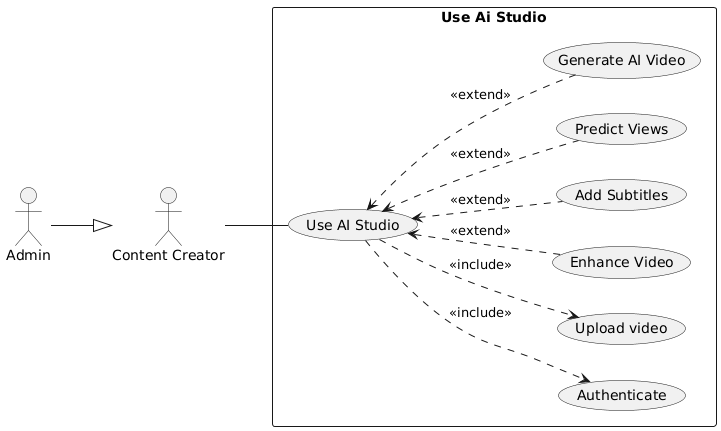
\includegraphics[width=0.65\textwidth]{diagram/diagram 5.png}
     \caption{Use case diagram of ``Alert Management''}
     \label{fig:uc-alerts}
 \end{figure}

\begin{table}[H]
\centering
\renewcommand{\arraystretch}{1.4}
\begin{tabular}{|p{4cm}|p{10cm}|}
\hline
\textbf{Title} & Use AI Studio \\ \hline

\textbf{Actor} & Content Creator / Admin \\ \hline

\textbf{Summary} & 
This use case allows the actor to access and use the AI Studio platform where they can upload videos, enhance content, generate AI videos, add subtitles, and predict video performance. \\ \hline

\textbf{Precondition} & 
The actor must be authenticated. \\ \hline

\textbf{Postcondition} & 
The actor successfully uses AI Studio features such as upload, enhancement, generation, and analytics. \\ \hline

\textbf{Main Scenario} & 
- The user accesses the AI Studio dashboard \newline
- The system authenticates the actor \newline
- The user must upload a video \newline
- The user can select an AI feature (enhance, subtitles, prediction, or generation) \\ \hline

\textbf{Alternative Scenario} & 
- Authentication failure \newline
- Upload failure due to unsupported format \newline
- AI processing error or timeout \newline
- Insufficient system resources for video generation \newline
- Invalid input parameters for AI processing \\ \hline

\end{tabular}
\caption{Use Case Description — Use AI Studio}
\label{tab:use-ai-studio}
\end{table}

\subsubsection*{Use Case Diagram: Admin Management}

In addition to the use cases shared with content creators, the administrator interacts with a dedicated set of supervisory features. These features were progressively added during the project (database migration \texttt{0006\_admin\_overhaul.sql}) to give the platform a real governance layer rather than a flat multi-tenant model.

\begin{table}[H]
\centering
\renewcommand{\arraystretch}{1.4}
\begin{tabular}{|p{4cm}|p{10cm}|}
\hline
\textbf{Title} & Admin Management \\ \hline

\textbf{Actor} & Admin \\ \hline

\textbf{Summary} &
This use case groups every administrator-only capability: governance of content creator accounts, oversight of all posts and videos across the platform, global analytics, soft-delete recovery (Trash), audit trail consultation, and operational monitoring of the job queues. \\ \hline

\textbf{Precondition} &
The actor must be authenticated and the resolved role from the Supabase JWT (claim \texttt{app\_role}) or the local user table must equal \texttt{admin}. \\ \hline

\textbf{Postcondition} &
The administrative action is executed, persisted, and a corresponding entry is written to the immutable admin audit log. \\ \hline

\textbf{Main Scenario} &
- The admin accesses the dedicated \texttt{/admin/*} routes through the dashboard sidebar \newline
- The backend re-checks the admin role via the \texttt{requireRole("admin")} Fastify decorator on every protected endpoint \newline
- The admin invites, edits, suspends, or removes a content creator from the Creators page \newline
- The admin browses every scheduled post or uploaded video across the whole platform (cross-tenant view) \newline
- The admin consults Global Analytics with filters, time ranges, and CSV export \newline
- The admin restores or permanently removes soft-deleted posts from the Trash page \newline
- The admin reviews the immutable audit trail of every administrative write \newline
- The admin monitors queue depth, failed jobs, and triggers one-click retries on the System Health page \newline
- The system records each write action into the \texttt{admin\_audit\_log} table \\ \hline

\textbf{Alternative Scenario} &
- The user is authenticated but does not hold the admin role: the API returns 403 Forbidden \newline
- The targeted account is already suspended or already deleted \newline
- A retried job ID no longer exists in the queue \newline
- The audit-log write fails (the original operation is still committed, but a warning is logged) \\ \hline

\end{tabular}
\caption{Use Case Description --- Admin Management}
\label{tab:admin-management}
\end{table}

\subsubsection*{Use Case Diagram: System Monitoring}

Beyond business-level oversight, the administrator also supervises the operational health of the platform. This use case formalises the System Health view and the retry workflow.

\begin{table}[H]
\centering
\renewcommand{\arraystretch}{1.4}
\begin{tabular}{|p{4cm}|p{10cm}|}
\hline
\textbf{Title} & System Monitoring \\ \hline

\textbf{Actor} & Admin \\ \hline

\textbf{Summary} &
This use case allows the administrator to inspect the runtime state of the four BullMQ queues (post-publishing, video-processing, analytics-refresh, ai-processing), browse failed jobs, and trigger a manual retry. \\ \hline

\textbf{Precondition} &
The actor must be authenticated as admin. Redis must be reachable and the API must be running. \\ \hline

\textbf{Postcondition} &
The selected job is re-enqueued. The retry action is recorded in the admin audit log under the \texttt{system.retry\_job} action. \\ \hline

\textbf{Main Scenario} &
- The admin opens the System Health page \newline
- The dashboard calls \texttt{GET /api/v1/admin/system/health} which aggregates job counts (waiting, active, completed, failed, delayed, paused) for each queue \newline
- The admin selects a queue and lists its failed jobs via \texttt{GET /api/v1/admin/system/failed-jobs?queue=...} \newline
- The admin clicks ``retry'' on a specific job, triggering \texttt{POST /system/jobs/:queue/:jobId/retry} \newline
- The system writes an audit entry and returns the new job state \\ \hline

\textbf{Alternative Scenario} &
- The queue name is invalid (validation error from the Zod schema) \newline
- The job ID no longer exists (404 Not Found) \newline
- Redis is unreachable (the System Health card displays a degraded state) \\ \hline

\end{tabular}
\caption{Use Case Description --- System Monitoring}
\label{tab:system-monitoring}
\end{table}

\subsection{Class Diagram}
The class diagram represents the data model of BViral Control Center. The main entities and their relationships are:

%\noindent\textit{See StarUML code --- Diagram 7 (Class Diagram).}

 \begin{figure}[H]
     \centering
     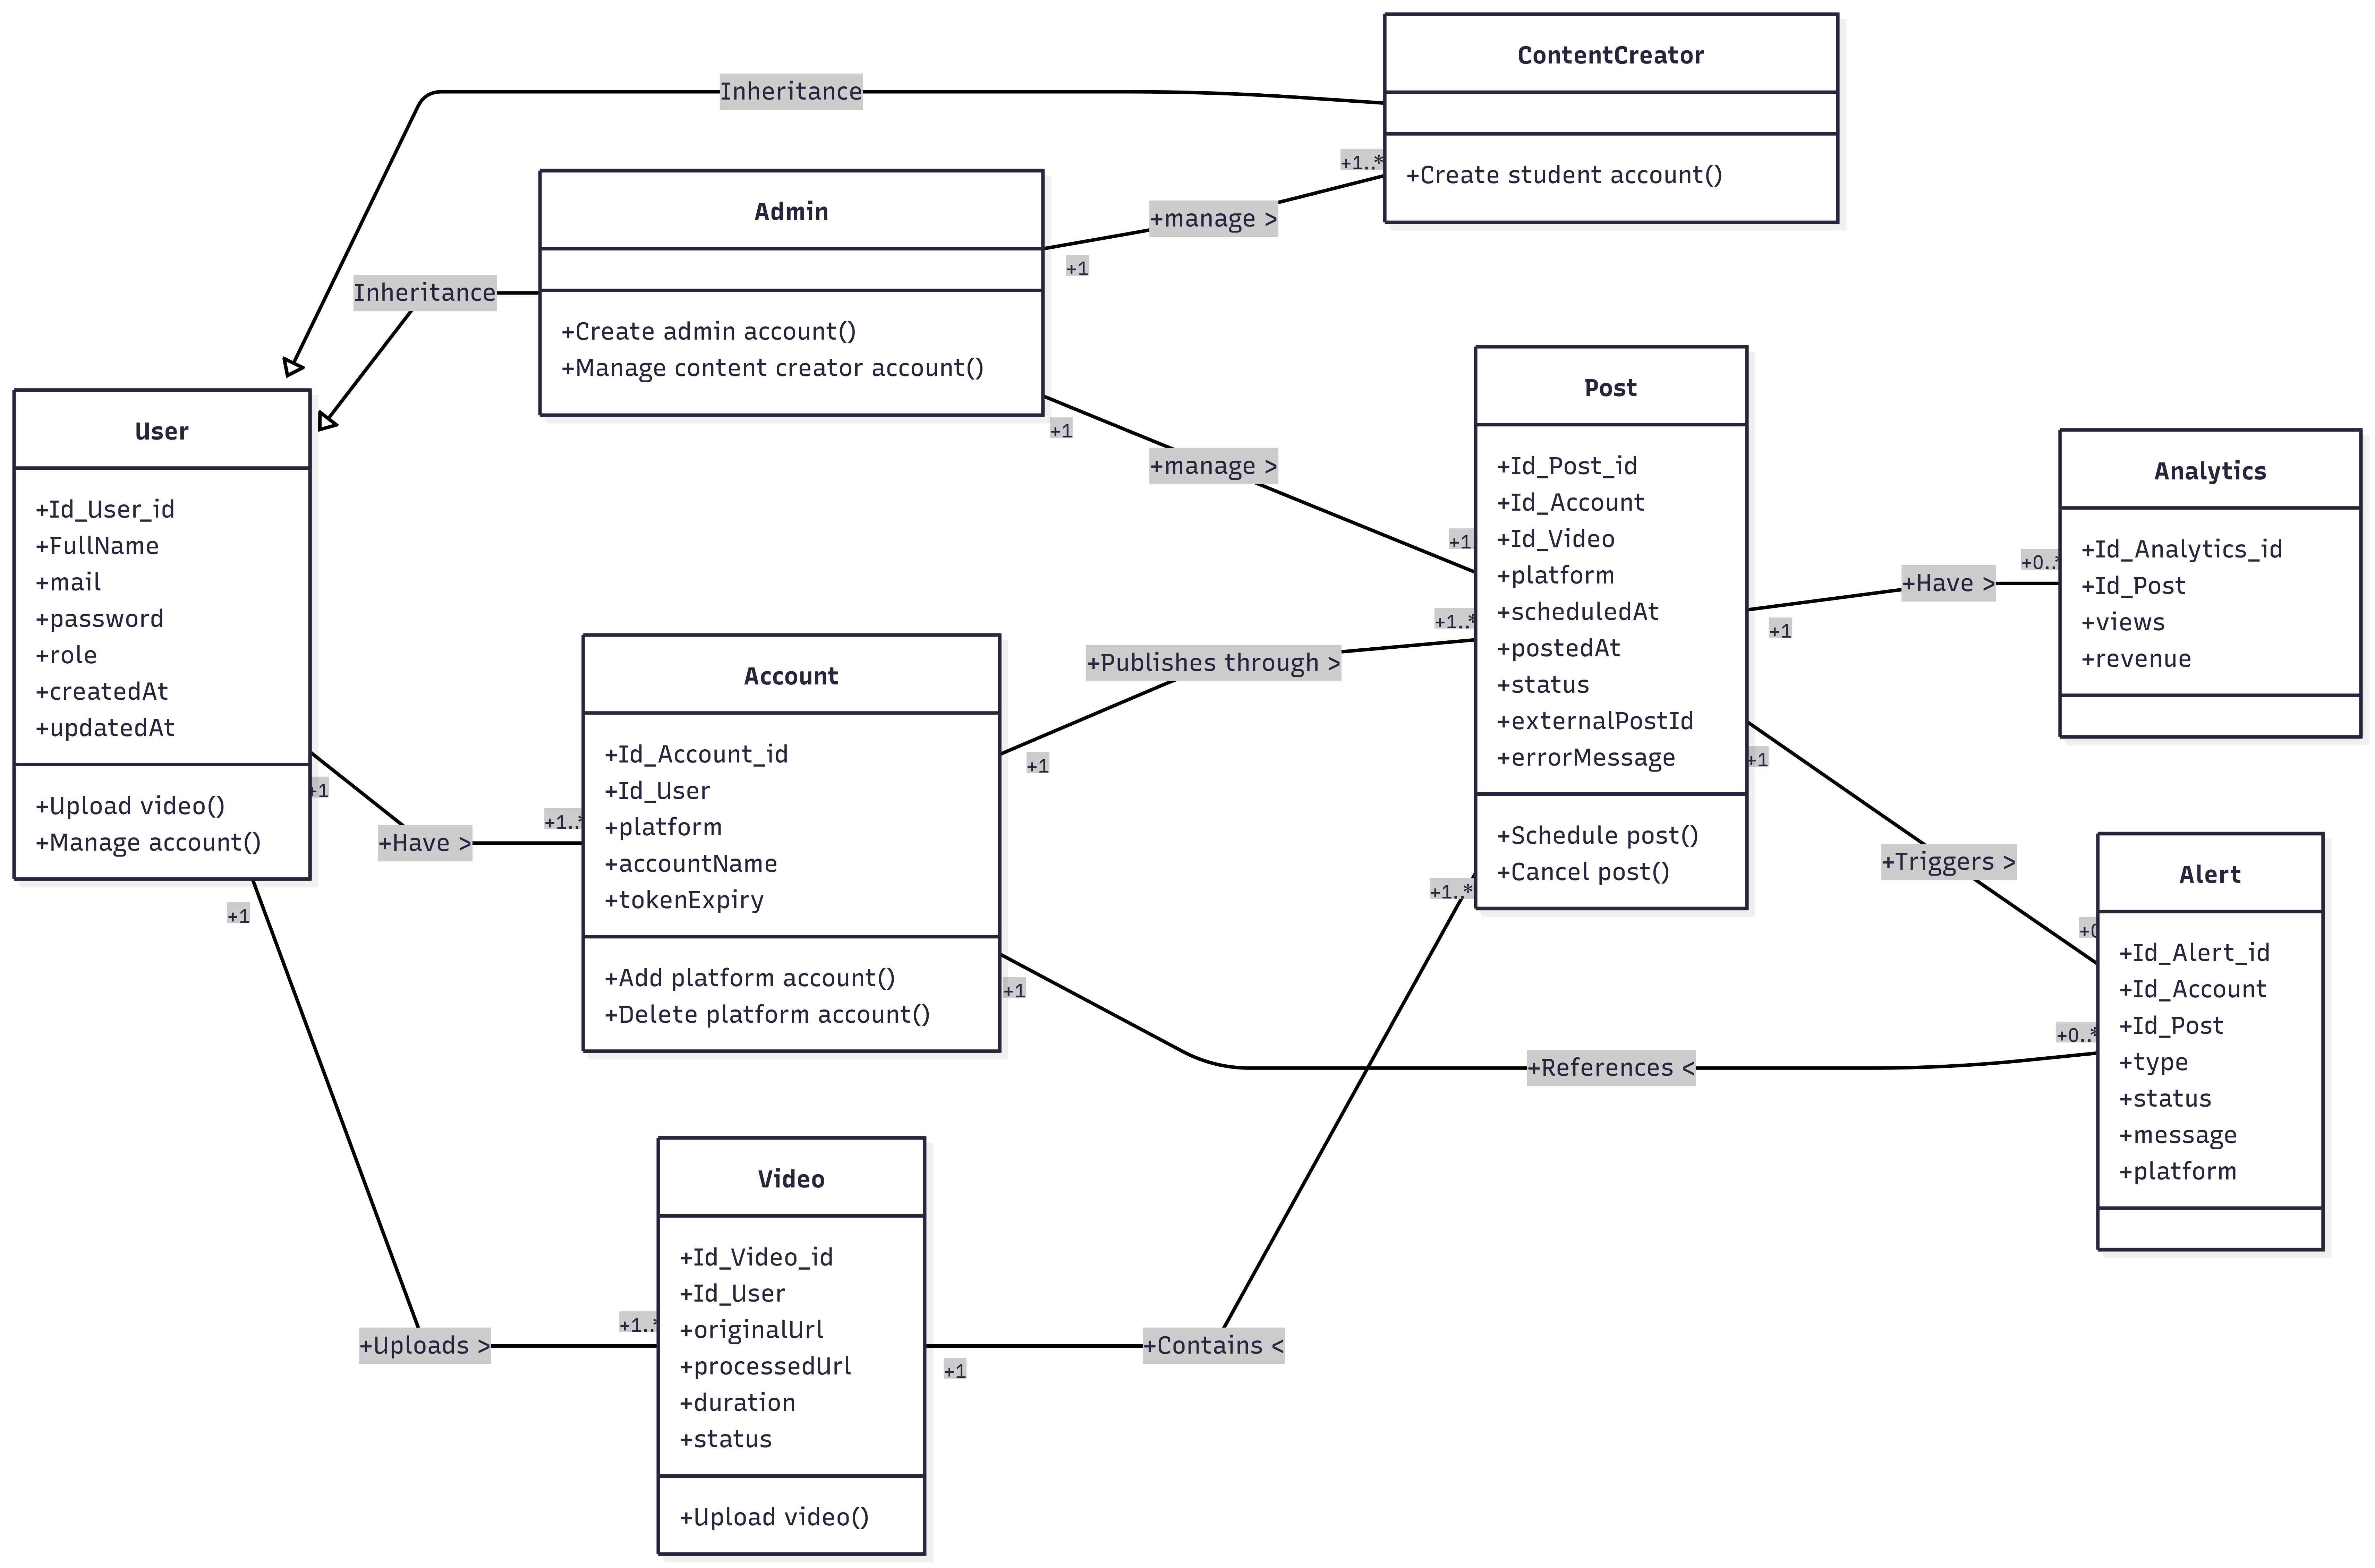
\includegraphics[width=\textwidth]{diagram/diagram class.png}
     \caption{Class diagram of BViral Control Center}
     \label{fig:class-diagram}
 \end{figure}

The system contains six main entities:
\begin{itemize}
    \item \textbf{User:} Represents a registered system user with attributes: \textit{Id\_User}, \textit{FullName}, \textit{mail}, \textit{password}, \textit{role}, \textit{createdAt}, and \textit{updatedAt}. It offers functionalities to \textit{Upload video()} and \textit{Manage account()}. It serves as the base class for two specialized roles:
    \begin{itemize}
        \item \textbf{ContentCreator:} Inherits from User and provides the capability to \textit{Create student account()}.
        \item \textbf{Admin:} Inherits from User and provides capabilities to \textit{Create admin account()} and \textit{Manage content creator account()}.
    \end{itemize}
    \item \textbf{Account:} Represents a linked platform account connected to a User, with attributes: \textit{Id\_Account\_id}, \textit{Id\_User}, \textit{platform}, \textit{accountName}, and \textit{tokenExpiry}. It handles functionalities to \textit{Add platform account()} and \textit{Delete platform account()}.
    \item \textbf{Video:} Represents a video asset uploaded by a User, with attributes: \textit{Id\_Video\_id}, \textit{Id\_User}, \textit{originalUrl}, \textit{processedUrl}, \textit{duration}, and \textit{status}. It includes an \textit{Upload video()} method.
    \item \textbf{Post:} Represents a scheduled or published publication linked to an Account and a Video, with attributes: \textit{Id\_Post\_id}, \textit{Id\_Account}, \textit{Id\_Video}, \textit{platform}, \textit{scheduledAt}, \textit{postedAt}, \textit{status}, \textit{externalPostId}, and \textit{errorMessage}. It handles functionalities to \textit{Schedule post()} and \textit{Cancel post()}.
    \item \textbf{Analytics:} Stores performance metrics linked to a specific Post, tracking: \textit{Id\_Analytics\_id}, \textit{Id\_Post}, \textit{views}, and \textit{revenue}.
    \item \textbf{Alert:} Represents system notifications triggered by posts or referenced by accounts, with attributes: \textit{Id\_Alert\_id}, \textit{Id\_Account}, \textit{Id\_Post}, \textit{type}, \textit{status}, \textit{message}, and \textit{platform}.
    \item \textbf{AdminAuditLog:} Immutable trace of every administrative write action, with attributes: \textit{Id\_AuditLog}, \textit{Id\_Admin}, \textit{action} (e.g.\ \texttt{system.retry\_job}, \texttt{creator.suspend}, \texttt{post.soft\_delete}), \textit{targetType}, \textit{targetId}, \textit{payload} (JSONB), and \textit{createdAt}. The table is indexed on \texttt{(adminId, createdAt)} and \texttt{(targetType, targetId)} for fast forensic queries.
\end{itemize}

\medskip
\noindent\textbf{Additional persistence-level attributes worth noting:}
\begin{itemize}
    \item The \textit{User} entity carries \textit{role} (\texttt{admin} or \texttt{content\_creator}), \textit{suspendedAt}, and \textit{suspendedBy} to support administrative governance.
    \item The \textit{Post} entity carries \textit{deletedAt} and \textit{deletedBy} to implement \emph{soft-delete} and the Trash recovery workflow.
    \item The \textit{Video} entity carries a \textit{contentHash} (SHA indexed on \texttt{(userId, contentHash)}) used to detect duplicate uploads.
    \item The \textit{Account} entity stores OAuth credentials (\textit{accessToken}, \textit{refreshToken}, \textit{tokenExpiry}). Tokens are persisted encrypted at rest using AES-256-GCM (see Chapter~3).
\end{itemize}


\textbf{Relationships:}
\begin{itemize}
    \item User $\xrightarrow{1..*}$ Account (a user owns multiple accounts)
    \item User $\xrightarrow{1..*}$ Video (a user uploads multiple videos)
    \item Account $\xrightarrow{1..*}$ Post (posts are published through accounts)
    \item Video $\xrightarrow{1..*}$ Post (a video can be posted to multiple platforms)
    \item Post $\xrightarrow{0..*}$ Analytics (each post has analytics snapshots)
    \item Account $\xrightarrow{0..*}$ Alert (alerts may reference an account)
    \item Post $\xrightarrow{0..*}$ Alert (alerts may reference a post)
\end{itemize}


\subsection{Sequence Diagrams}



\subsubsection{Sequence Diagram: Authentification}
%\noindent\textit{See StarUML code --- Diagram 8.}

 \begin{figure}[H]
     \centering
     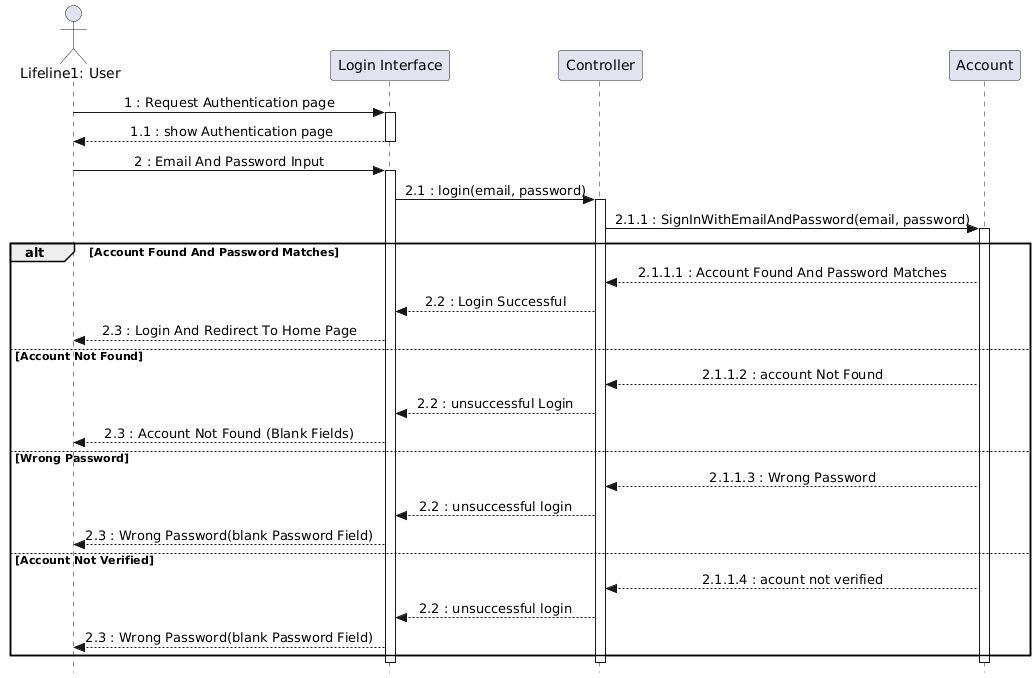
\includegraphics[width=\textwidth]{diagram/diagramme sequence 1.png}
     \caption{Sequence diagram of Authentification}
     \label{fig:seq-oauth}
 \end{figure}

\begin{enumerate}
    \item The user requests the authentication page via the login interface to access the application dashboard.
    \item The user inputs their credentials, specifying their email and password, into the login form.
    \item The login interface transmits the credentials to the backend application layer by invoking the login handler.
    \item The controller authenticates the submission details by requesting a lookup from the core account management service.
    \item The account service verifies the credentials against the identity database, checking for user existence, password matches, and verification flags.
    \item On success, the account confirmation is returned to the interface, which authenticates the session and redirects the user to the application home page.
    \item On validation failure (such as account not found, incorrect password, or unverified profile status), an unsuccessful login status is returned, displaying a precise error message to the interface.
\end{enumerate}

\subsubsection{Sequence Diagram: Post Scheduling}
%\noindent\textit{See StarUML code --- Diagram 9.}

 \begin{figure}[H]
     \centering
     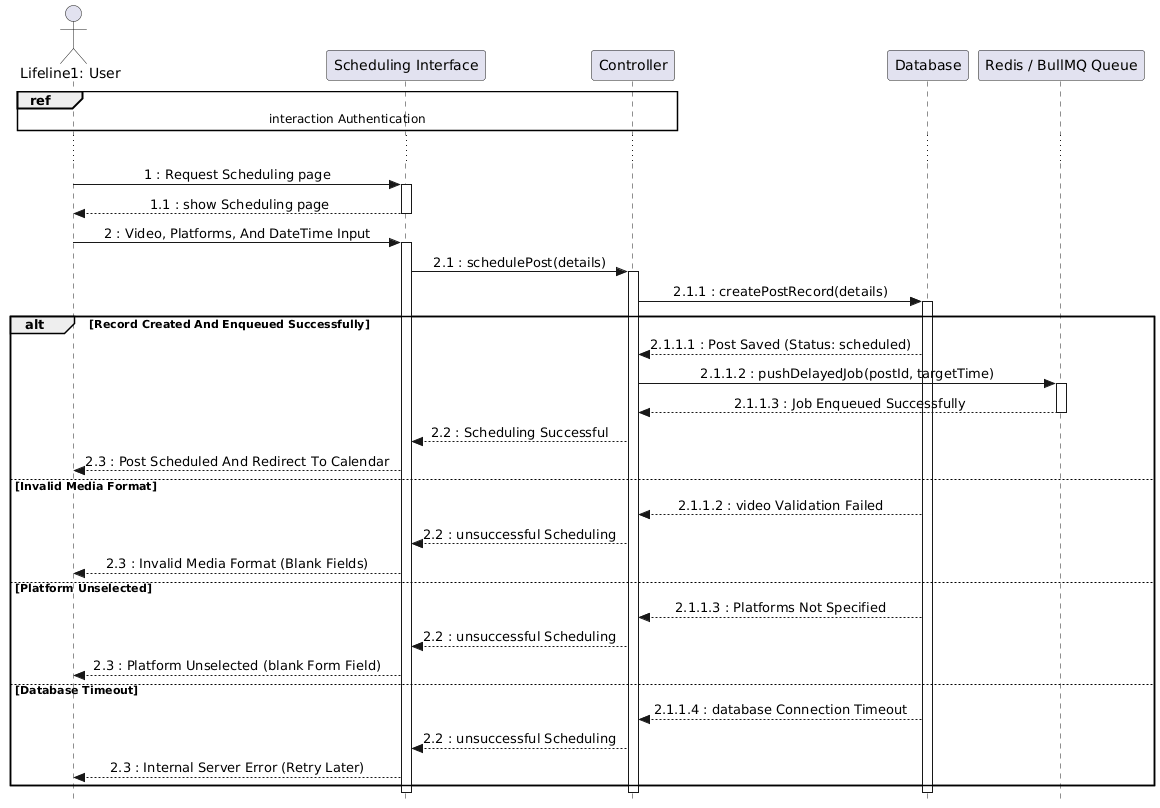
\includegraphics[width=\textwidth]{diagram/diagramme sequence 2.png}
     \caption{Sequence diagram of ``Schedule and Publish a Post''}
     \label{fig:seq-schedule}
 \end{figure}

The scheduling and publishing flow:
\begin{enumerate}
    \item The user creates a new post in the scheduling interface, selecting video, platform, account, and schedule time.
    \item The dashboard sends a POST request to \texttt{/api/v1/posts}.
    \item The API server validates the request, creates a post record with status ``scheduled'', and enqueues a delayed job in the Redis/BullMQ publishing queue.
    \item At the scheduled time, the BullMQ worker dequeues the job.
    \item The worker calls the appropriate platform publisher service (YouTube, TikTok, or Meta).
    \item The platform service uploads the video and metadata using the stored OAuth tokens.
    \item On success, the post status is updated to ``posted'' with the external post ID. On failure, it is marked ``failed'' with an error message, and an alert is created.
\end{enumerate}

\section{AI Pipeline Specification \& Processing Steps}

The analytical method follows a strict end-to-end Machine Learning pipeline, summarized in Figure~\ref{fig:ai-workflow-diagram}.

\begin{figure}[H]
    \centering
    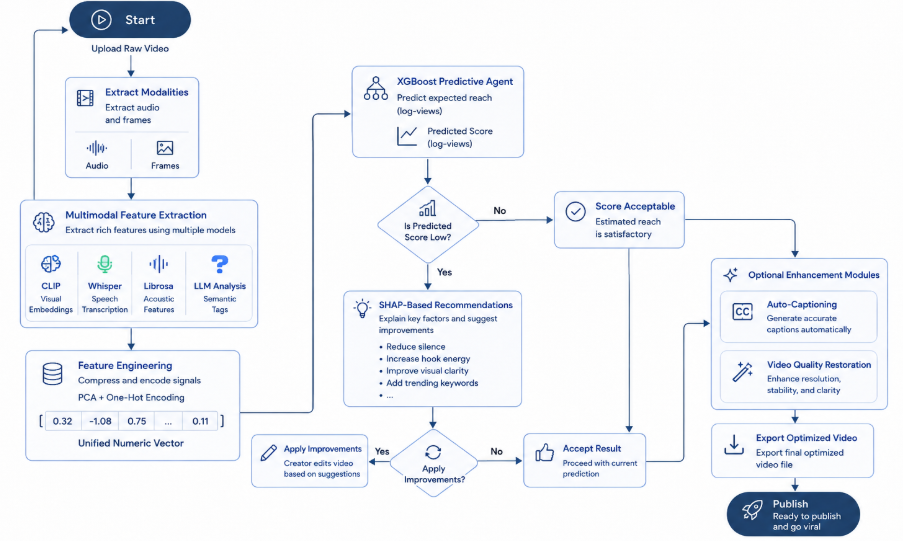
\includegraphics[width=0.9\textwidth]{images/0workflowdiagram.png}
    \caption{Workflow diagram of the AI pipeline and processing steps}
    \label{fig:ai-workflow-diagram}
\end{figure}
\begin{enumerate}
    \item \textbf{Data Ingestion:} Raw \texttt{.mp4} videos are uploaded and split into audio (\texttt{.wav}) and video frames using \texttt{FFmpeg}.
    \item \textbf{Feature Extraction \& Preprocessing:} Multimodal foundation models (CLIP, Librosa, Whisper, Llama 3) extract high-dimensional semantic data.
    \item \textbf{Feature Engineering:} Principal Component Analysis (PCA) compresses the dense vectors (e.g., 512D to 64D) to prevent overfitting. Categorical LLM tags are One-Hot Encoded.
    \item \textbf{Model Training:} The final 473-dimensional vector is fed into the XGBoost Regressor to map content features to the \texttt{log\_views} target.
    \item \textbf{Evaluation \& XAI:} The model is evaluated using RMSE and $R^2$. SHAP (SHapley Additive exPlanations) is applied to extract actionable feedback.
    \item \textbf{Deployment:} The trained model, scalers, and PCA transformers are exported via \texttt{pickle} for integration into the final application.
\end{enumerate}



\section*{Conclusion}
\phantomsection
\addcontentsline{toc}{section}{Conclusion}
In this chapter, we analyzed and modeled the functional and structural requirements of the BViral Control Center platform. Use-case diagrams and detailed scenarios were used to describe the interactions between users and the system, while the class diagram defined the main entities and their relationships. Sequence diagrams illustrated the dynamic behavior of key processes such as authentication and post scheduling. Finally, the AI pipeline specification presented the workflow of the intelligent video processing and prediction system. These analyses provide a solid foundation for the implementation phase discussed in the next chapter.